\documentclass{article}

\usepackage{tikz}
\usetikzlibrary{automata, positioning}
\begin{document}
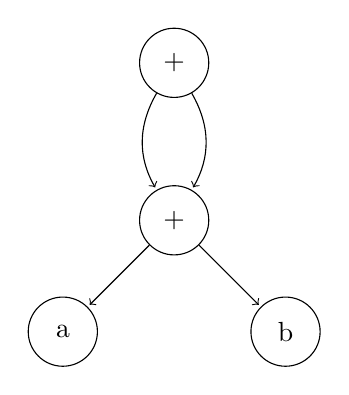
\begin{tikzpicture}[shorten >= 1pt, node distance = 2cm, on grid, auto]
  \node[state] (4) {+};
  \node[state] (3) [below=of 4] {+};
  \node[state] (1) [below left=of 3] {a};
  \node[state] (2) [below right=of 3] {b};
  \path[->]
    (4) edge [bend right] node {} (3)
        edge [bend left] node {} (3)
    (3) edge node {} (2)
        edge node {} (1);
\end{tikzpicture}
\end{document}
